\documentclass[11pt,a4paper]{report}
\usepackage[margin=2.5cm]{geometry}
\usepackage[T1]{fontenc}
\usepackage{amsmath,amssymb}
\usepackage{graphicx}
\usepackage{booktabs}
\usepackage{enumitem}
\usepackage[hidelinks]{hyperref}

\begin{document}

% ---- Title page: replace the title, authors, organisation and date. ----
\begin{titlepage}
  \centering
  \vspace*{3cm}
  {\Huge\bfseries Campus Bike-Share Pilot\par}
  \vspace{0.6cm}
  {\LARGE Final Evaluation Report\par}
  \vspace{2.5cm}
  {\Large Maya Oyelaran \quad Felix Brauer \quad Chen Jing\par}
  \vspace{0.6cm}
  {\large Sustainable Transport Office\\Riverside University\par}
  \vfill
  {\large Prepared for the University Estates Committee\par}
  \vspace{0.4cm}
  {\large 14 March 2026\par}
\end{titlepage}

\pagenumbering{roman}

% ---- Abstract: replace with a one-paragraph summary of the whole report. ----
\begin{abstract}
Between March and August 2025 Riverside University ran a pilot bike-share scheme with 120 bicycles at eight docking stations. This report evaluates the pilot against the three goals set by the Estates Committee: use, cost and effect on car travel to campus. Members made 71\,460 trips, an average of 3.3 trips per bicycle per day, and use grew in every month except June and July, when teaching stopped. The scheme cost 2.10 per trip after membership income, which is below the 2.50 target. A survey of 412 members indicates that 14\% of trips replaced a car journey. We recommend extending the scheme to 200 bicycles and twelve stations, and moving two stations that saw little use.
\end{abstract}

\tableofcontents
\listoffigures
\listoftables

\clearpage
\pagenumbering{arabic}

% ---- Chapters: one file each in chapters/. Add a chapter by adding a file and an \input line. ----
\chapter{Introduction}\label{ch:introduction}

\section{Purpose of the Report}
In November 2024 the University Estates Committee approved a six-month pilot of a bike-share scheme on the main campus and asked the Sustainable Transport Office to report on its results. This document is that report. It is intended to give the Committee what it needs to decide whether the scheme should end, continue as it is, or be extended.

\section{The Pilot in Brief}
The pilot ran from 3 March to 31 August 2025. It provided 120 bicycles at eight docking stations: six on the main campus, one at the railway station and one at the Northgate student residences. Staff and students could join for a flat fee per term, which covered every trip of up to 45 minutes.

\section{Goals Set by the Committee}\label{sec:goals}
The Committee set three goals, each with a measurable target:
\begin{enumerate}[label=\textbf{G\arabic*}]
  \item \textbf{Use.} An average of at least 2.5 trips per bicycle per day over the pilot.
  \item \textbf{Cost.} A net cost to the University of no more than 2.50 per trip.
  \item \textbf{Car travel.} At least 10\% of trips replacing a journey that would otherwise have been made by car.
\end{enumerate}

\section{Structure of the Report}
Chapter~\ref{ch:background} summarises what is known about bike-share schemes at other institutions. Chapter~\ref{ch:methods} describes the data and how each goal was measured. Chapter~\ref{ch:results} presents the results, and Chapter~\ref{ch:recommendations} gives our recommendations. The survey questions are reproduced in Appendix~\ref{app:survey}.

\chapter{Background}\label{ch:background}

\section{Bike-Share Schemes}
Public bike-share schemes have spread to more than a thousand cities since the mid-2000s. Reviews of the research agree on two points \cite{fishman2013bike,shaheen2010bikesharing}. First, use depends heavily on how close stations are to where people start and end their journeys. Second, most trips replace walking or public transport rather than driving, so the effect on car travel is real but smaller than scheme operators tend to claim.

\section{What Influences Use}
A study of the scheme in Washington, DC, found that trips rose with temperature up to about 30 degrees and fell sharply in rain, and that stations near public transport were used more \cite{gebhart2014impact}. University schemes add a strong calendar effect, because most members leave during vacations.

\section{Lessons for This Pilot}
Three lessons shaped the design of the pilot:
\begin{itemize}
  \item stations were placed at the two ends of the most common walking journeys, not spread evenly;
  \item one station was placed at the railway station, to connect with public transport;
  \item the survey asked directly which mode each trip replaced, so that the effect on car travel would not have to be inferred.
\end{itemize}

\chapter{Methods}\label{ch:methods}

\section{Overview}
Figure~\ref{fig:method} shows the steps of the evaluation. Trip records and survey answers were collected throughout the pilot, checked, analysed against the three goals, and reviewed with the scheme operator before this report was written.

\begin{figure}[htbp]
  \centering
  % Replace with your own figure: upload an image and change the file name below.
  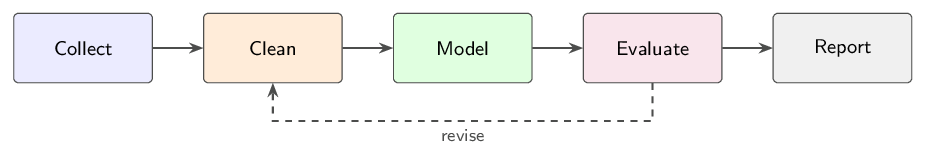
\includegraphics[width=0.9\textwidth]{figures/method.png}
  \caption{Steps of the evaluation.}
  \label{fig:method}
\end{figure}

\section{Trip Data}
Every docking station records the time at which a bicycle is released and returned. We received 73\,912 trip records from the operator. Records shorter than one minute or returned to the same station within three minutes were treated as failed releases and removed, which left 71\,460 trips.

\section{Measuring Use}
Use is reported as trips per bicycle per day,
\begin{equation}\label{eq:use}
  u = \frac{N}{B \times D},
\end{equation}
where $N$ is the number of trips, $B$ the number of bicycles in service and $D$ the number of days. Over the pilot, $B = 120$ and $D = 182$.

\section{Measuring Cost}
The net cost per trip is the operating cost less membership income, divided by the number of trips:
\begin{equation}\label{eq:cost}
  c = \frac{C_{\mathrm{op}} - I}{N}.
\end{equation}
Operating cost includes the operator's fee, maintenance and staff time. The purchase of bicycles and stations was funded by a separate grant and is not included.

\section{Survey}
All 1\,846 members were invited by email to complete a short survey in the final two weeks of the pilot; 412 did so, a response rate of 22\%. The key question asked how the respondent would have made their most recent trip if the scheme had not existed.

\chapter{Results}\label{ch:results}

\section{Use}
Members made 71\,460 trips. By Equation~\eqref{eq:use} this is
\[
  u = \frac{71\,460}{120 \times 182} \approx 3.3
\]
trips per bicycle per day, above the target of 2.5. Figure~\ref{fig:trips} shows average daily trips by month. Weekday use rose steadily until May, dipped in June and July when teaching stopped, and reached its highest level in August as students returned. Weekend use grew in every month.

\begin{figure}[htbp]
  \centering
  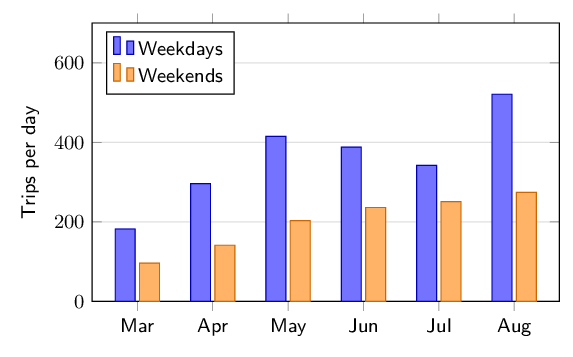
\includegraphics[width=0.75\textwidth]{figures/daily-trips.png}
  \caption{Average trips per day by month, for weekdays and weekends.}
  \label{fig:trips}
\end{figure}

Use was uneven between stations, as Table~\ref{tab:stations} shows. The Library and the railway station together accounted for 42\% of all trips, while Sports Centre and East Gate accounted for 7\%.

\begin{table}[htbp]
  \centering
  \caption{Trips starting at each station over the pilot.}
  \label{tab:stations}
  \begin{tabular}{lrr}
    \toprule
    Station & Trips & Share (\%) \\
    \midrule
    Library            & 16\,150 & 22.6 \\
    Railway station    & 13\,862 & 19.4 \\
    Northgate          & 11\,720 & 16.4 \\
    Science Quarter    & 10\,290 & 14.4 \\
    Students' Union    &  8\,504 & 11.9 \\
    Main Building      &  5\,932 &  8.3 \\
    Sports Centre      &  2\,858 &  4.0 \\
    East Gate          &  2\,144 &  3.0 \\
    \midrule
    Total              & 71\,460 & 100.0 \\
    \bottomrule
  \end{tabular}
\end{table}

\section{Cost}
Table~\ref{tab:cost} sets out income and costs. By Equation~\eqref{eq:cost} the net cost was 2.10 per trip, below the target of 2.50.

\begin{table}[htbp]
  \centering
  \caption{Operating cost and income over the pilot.}
  \label{tab:cost}
  \begin{tabular}{lr}
    \toprule
    Item & Amount \\
    \midrule
    Operator's fee            & 132\,000 \\
    Maintenance and repairs   &  31\,400 \\
    Staff time                &  23\,960 \\
    \midrule
    Total operating cost      & 187\,360 \\
    Membership income         &  37\,294 \\
    \midrule
    Net cost                  & 150\,066 \\
    Net cost per trip         &     2.10 \\
    \bottomrule
  \end{tabular}
\end{table}

\section{Effect on Car Travel}
Of the 412 survey respondents, 58 (14\%) said that their most recent trip would otherwise have been made by car, as driver or passenger. A further 201 (49\%) would have walked, 117 (28\%) would have taken a bus and 36 (9\%) would not have made the trip. The 14\% figure meets the target of 10\%. Because people who responded may differ from those who did not, we treat it as an estimate with a margin of roughly three percentage points either way.

\section{Summary Against the Goals}
All three goals in Section~\ref{sec:goals} were met: 3.3 trips per bicycle per day against a target of 2.5, a net cost of 2.10 per trip against 2.50, and 14\% of trips replacing a car journey against 10\%.

\chapter{Recommendations}\label{ch:recommendations}

\section{Continue and Extend the Scheme}
The pilot met its three goals, and use was still growing when it ended. We recommend that the scheme continues and is extended from 120 to 200 bicycles and from eight to twelve stations, with the new stations at the Medical School, the West Car Park, Riverside Halls and the city-centre teaching building.

\section{Move the Two Least-Used Stations}
Sports Centre and East Gate together produced 7\% of trips. Both are within 250 metres of a busier station. We recommend moving them to the Engineering Workshops and the Park-and-Ride stop, which were the two locations most often requested in the survey.

\section{Review After One Academic Year}
The pilot did not include a winter. Studies elsewhere suggest that use will fall in cold and wet months \cite{gebhart2014impact}. We recommend that the Committee reviews use and cost again in September 2026, with a full year of data.

\section{Risks}
\begin{itemize}
  \item \textbf{Winter use.} If winter use falls below 1.5 trips per bicycle per day, the net cost per trip for the year would exceed the 2.50 target.
  \item \textbf{Operator's fee.} The current fee is fixed until August 2026 and may rise afterwards.
  \item \textbf{Survey bias.} The estimate of car trips replaced rests on a 22\% response rate.
\end{itemize}


\appendix
\chapter{Member Survey}\label{app:survey}

The survey was open from 18 to 31 August 2025. The questions are reproduced below.

\begin{enumerate}
  \item How often did you use the bike-share scheme during the pilot? \emph{(Most days / A few times a week / A few times a month / Less often)}
  \item Thinking about your most recent trip, where did it start and end?
  \item If the scheme had not existed, how would you have made that trip? \emph{(Walked / Bus / Car as driver / Car as passenger / Own bicycle / Would not have made the trip)}
  \item How satisfied are you with the availability of bicycles at the station you use most? \emph{(1 = very dissatisfied, 5 = very satisfied)}
  \item Where would you most like a new station?
  \item Is there anything else you would like to tell us?
\end{enumerate}

\section{Response Summary}
Table~\ref{tab:survey} gives the number of responses by group.

\begin{table}[htbp]
  \centering
  \caption{Survey invitations and responses by member group.}
  \label{tab:survey}
  \begin{tabular}{lrrr}
    \toprule
    Group & Invited & Responded & Rate (\%) \\
    \midrule
    Undergraduate students & 1\,104 & 221 & 20 \\
    Postgraduate students  &    398 &  97 & 24 \\
    Staff                  &    344 &  94 & 27 \\
    \midrule
    All members            & 1\,846 & 412 & 22 \\
    \bottomrule
  \end{tabular}
\end{table}


\bibliographystyle{plain}
\bibliography{references}

\end{document}
